\chapter{Usability, Security, Safety and Energy Efficiency \\
\small{\textit{-- ZKD, KRV, CL, \& ZZ}}
\index{Usability, Security, Safety and Energy Efficiency} 
\index{Chapter!Usability}
\label{Chapter::Usability}}

\textbf{Context:} The oscilloscope is networked and shares data with labs that may be interested in remote monitoring of voltages.  The oscilloscope has a Wi-Fi and cellular connection.

\begin{figure}[h]
    \centering
    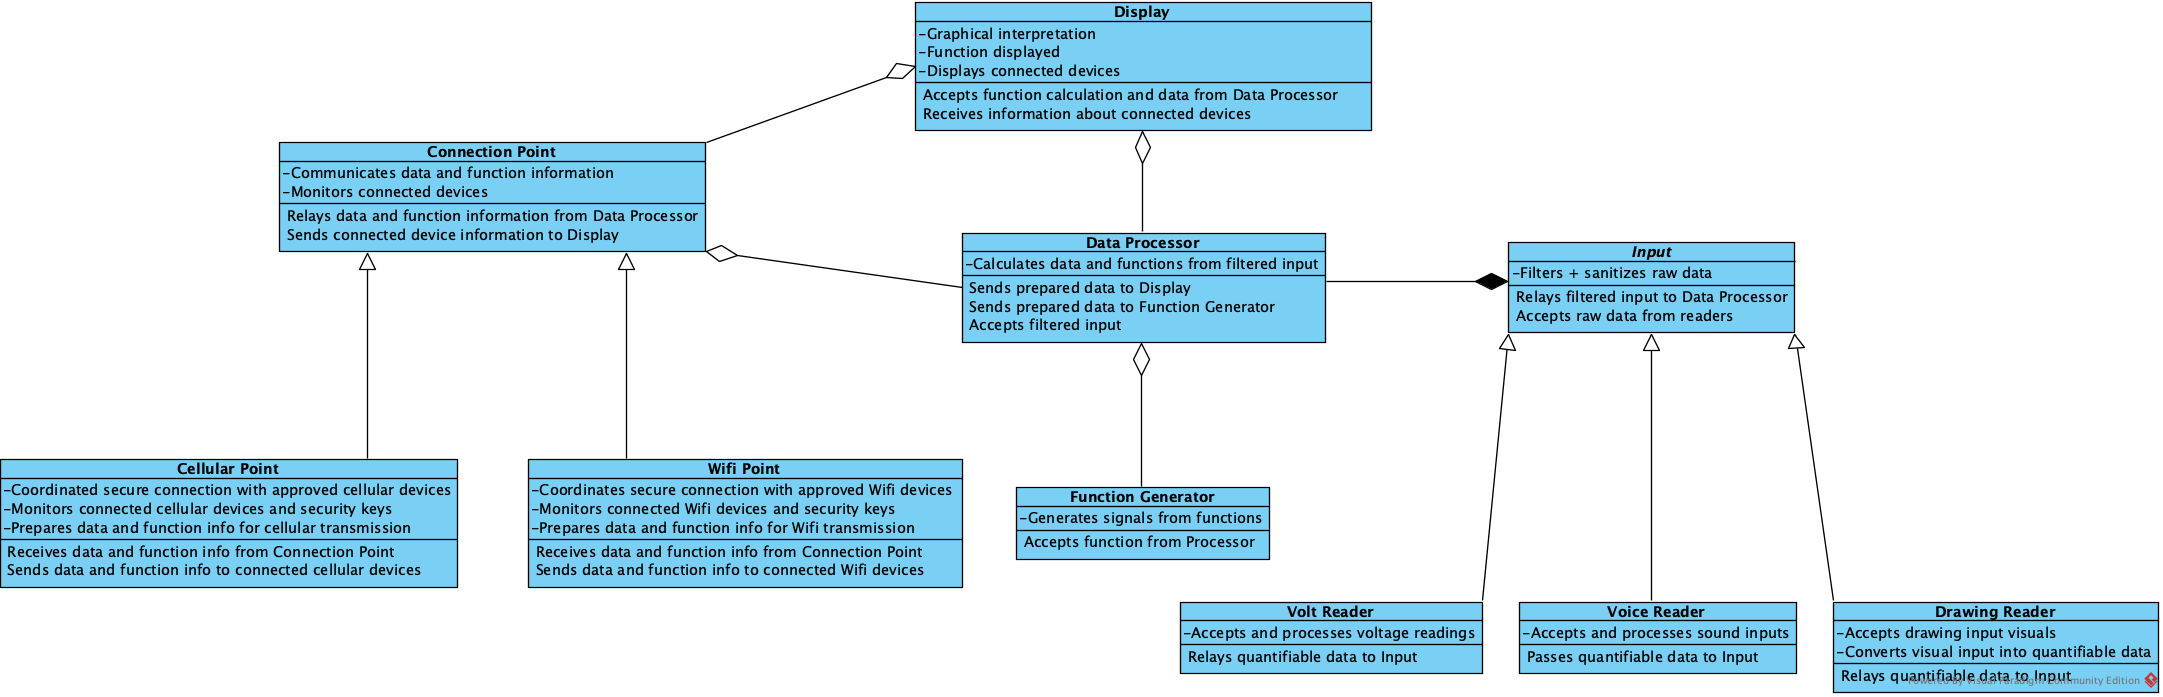
\includegraphics[scale=0.4]{Book-SSW565/png/Scope-Function-Generator-2.png}
    \caption{\label{Figure::Oscilloscope Class Diagram}Oscilloscope Class Diagram}
\end{figure}

\section{Usability Scenario}

\begin{longtable}{|l|p{12cm}|}
%\centering
\caption{\TableName{Usability Scenario for Oscilloscope} \TableLabel{USOscilloscope} \label{Table::UsabilityOscilloscope}}\\
    
    \hline
    \textbf{Portion} & \textbf{Possible Values}\\
    \hline 
    \endfirsthead

    \multicolumn{2}{c}{\tablename\ \thetable\ -- \textit{Continued from previous page}}\\
    \hline
    \textbf{Portion} & \textbf{Possible Values}\\
    \hline
    \endhead
    
    \multicolumn{2}{r}{\tablename\ \thetable\ -- \textit{Continued on next page}} \\
    \endfoot
    \endlastfoot

\gls{stakeholder} & Lab Engineer / Technician
\\ \hline

\gls{source} & The engineer initiates the action via a web-based interface or a mobile app connected to the oscilloscope.
\\ \hline

\gls{stimulus} & The engineer logs in and selects the volt reader function, then modifies the voltage either Vertical scale (volts per division) or Vertical scale (volts per division).
\\ \hline

\gls{environment} & The oscilloscope is in a networked lab environment, accessed remotely by Wi-Fi or cellular network.
\\ \hline

\gls{artifact} & The oscilloscope system, including the Wi-Fi Point, Cellular Point, Volt Reader, and Data Processor, which must authenticate the user before allowing adjustments.
\\ \hline

\gls{response} & The oscilloscope authenticates the user, then applies the voltage change, updating the display with the new settings.
\\ \hline

\gls{responseMeasure} & Authentication time less than and equal to 15 sec \\
     & Voltage adjustment processing time less than and equal to 5 sec \\
     & Total time for task completion less than and equal to 20 sec
\\ \hline

\end{longtable}
An engineer remotely accesses the networked oscilloscope, requiring authentication before voltage settings can be altered. The system then processes the change and updates the display. Performance is measured by total interaction time and system response speed.

\section{Usability Trade-offs}
While usability is a great improvement to any software, the trade-offs of such need to be considered in the full scope of the system. Depending on the system and its trade-offs, the developers need to find a healthy balance.

\subsection{Against Security}
The trade-off between usability and security tends to be that as the software gets more user friendly, detailed options might start to be removed for the user's experience which can lead to a less secure connection. Think of it this way, the easier it is for someone to connect their device to the oscilloscope, the easier it is for anyone to connect their device to that same oscilloscope and read all the data being transmitted. While yes, the oscilloscope has become easier to use, it also compromises the possible sensitive data from the device or the other devices connected to it. 
\paragraph{\textbf{The above-mentioned scenario significantly impacts security:}}
\begin{itemize}
    \item Without authentication: Instant access (around ~5 sec).
    \item With authentication: Extra 10-15 sec before access.
\end{itemize}

\begin{table}[htbp]
\centering
\caption{Usability, Security, and Access Time Comparison}
\resizebox{\textwidth}{!}{
\begin{tabular}{|l|c|c|c|} % Added vertical bars
\hline % Added top border
\textbf{Scenario} & \textbf{Usability Impact} & \textbf{Security Benefit} & \textbf{Access Time} \\
\hline % Added horizontal line
No Authentication & Fast access (around 5 sec) & Unprotected, anyone can access & around 5 sec \\
\hline
Authentication Required & Slower access (15-20 sec) & Secure, only authorized users & 15-20 sec \\
\hline % Added bottom border
\end{tabular}}
\label{tab:security_usability}
\end{table}

\paragraph{\textbf{Solution of above trade-offs:}}
 Implement a "Remember Me" feature to reduce login time for returning users.

\subsection{Against Performance}
Trade-offs between usability and performance may system from a developer's desire to keep the oscilloscope very simple to use while still accounting for all possible use cases of said machine. That means that while the user might only want to read the voltage of something and have it displayed on the Display, the software might take all possible functions and features into account, such as preparing that data for WiFi transmission, which compromise performance. 

\paragraph{\textbf{The above-mentioned scenario significantly impacts performance:}}
\begin{itemize}
    \item If oscilloscope encrypts data before sending via Wi-Fi, it might delay response times by 1-2 sec.
    \item If Data Processor filters raw input before calculation, it ensures accuracy but adds processing time.
\end{itemize}
\paragraph{\textbf{Solution through Optimization:}}Perform real-time processing in parallel with data transmission.

\section{Requirements}

\subsection{Requirement 1: Voltage Measurement and Adjustment}
The oscilloscope must provide precise \textbf{voltage measurement} and allow users to adjust the \textbf{either Vertical scale (volts per division) or Vertical scale (volts per division).} remotely via a web-based interface or mobile app.

\paragraph{\textbf{Usability Response:}}  
The oscilloscope authenticates the user, then applies the voltage change, updating the display with the new settings.

\paragraph{\textbf{Response Measure:}}  
\begin{itemize}
    \item Authentication time: $\leq 15$ seconds.
    \item Voltage adjustment processing time: $\leq 5$ seconds.
    \item Total task completion time: $\leq 20$ seconds.
\end{itemize}

\paragraph{\textbf{Comparison of Usability:}}  
Compared to traditional oscilloscopes, which require physical interaction for voltage adjustments, this remote-controlled oscilloscope improves usability by allowing engineers to make real-time changes from anywhere. The inclusion of authentication ensures security, but it adds a minor delay in response time. The \textbf{automated process reduces human error} while maintaining efficiency.

\subsection{Requirement 2: Frequency Measurement and Remote Monitoring}
The oscilloscope must allow users to measure \textbf{signal frequency} and remotely monitor real-time waveforms over Wi-Fi and cellular networks.

\paragraph{\textbf{Usability Response:}}  
The oscilloscope captures and transmits frequency data to remote users, allowing them to view measurements in real-time.

\paragraph{\textbf{Response Measure:}}  
\begin{itemize}
    \item Frequency detection processing time: $\leq 10$ milliseconds.
    \item Data transmission time to remote labs: $\leq 3$ seconds.
    \item Display update interval: $\leq 1$ second.
\end{itemize}

\paragraph{\textbf{Comparison of Usability:}}  
Traditional oscilloscopes require engineers to be physically present for monitoring. The ability to view frequency readings remotely enhances usability by allowing multiple users to access data from different locations. However, data transmission over a network introduces slight latency, which could be an issue in high-precision applications.  

\section{Energy Trade-offs}

\paragraph{\textbf{Wi-Fi Point:}}  
\begin{itemize}
    \item Lower power consumption compared to cellular.
    \item Requires authentication for every new session, adding a slight delay.
    \item More stable connection in controlled lab environments.
    \item Limited range, requiring the user to be within the Wi-Fi coverage area.
\end{itemize}

\paragraph{\textbf{Cellular Point:}}  
\begin{itemize}
    \item Higher power consumption due to continuous network communication.
    \item Allows persistent connections, reducing the need for frequent re-authentication.
    \item Greater range, enabling remote access from anywhere with a cellular network.
    \item Potential latency issues, depending on network conditions.
\end{itemize}

\paragraph{\textbf{Define better way to improve energy efficiency:}}  
\begin{itemize}
    \item Use Wi-Fi for frequent, short-duration access to conserve energy.
    \item Use Cellular for long-term remote monitoring where stability and persistent access are prioritized.
    \item Implement adaptive authentication (e.g., session-based authentication caching) to balance usability, security, and energy efficiency.
\end{itemize}



